\documentclass[border=6pt]{standalone}
\usepackage{tikz}
\usepackage[edges]{forest}
\usetikzlibrary{arrows.meta,positioning,calc,decorations.pathreplacing,shapes.geometric}
\begin{document}
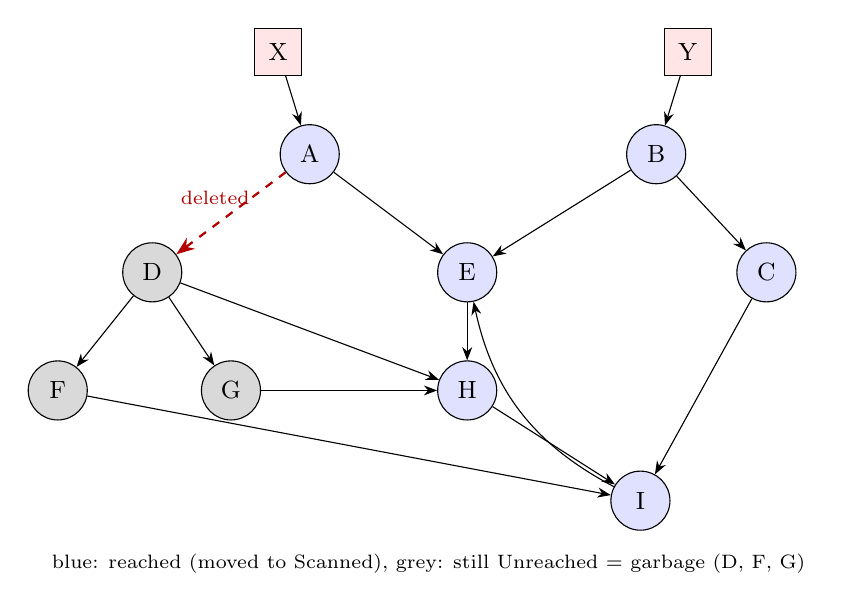
\begin{tikzpicture}[>=Stealth,font=\small,v/.style={draw,circle,minimum size=0.75cm,inner sep=0pt},r/.style={draw,rectangle,fill=red!10,minimum size=0.6cm,inner sep=1pt}]
\node[r] (X) at (0.00,4.20) {X};
\node[r] (Y) at (5.20,4.20) {Y};
\node[v,fill=blue!12] (A) at (0.40,2.90) {A};
\node[v,fill=blue!12] (B) at (4.80,2.90) {B};
\node[v,fill=gray!30] (D) at (-1.60,1.40) {D};
\node[v,fill=blue!12] (E) at (2.40,1.40) {E};
\node[v,fill=blue!12] (C) at (6.20,1.40) {C};
\node[v,fill=gray!30] (F) at (-2.80,-0.10) {F};
\node[v,fill=gray!30] (G) at (-0.60,-0.10) {G};
\node[v,fill=blue!12] (H) at (2.40,-0.10) {H};
\node[v,fill=blue!12] (I) at (4.60,-1.50) {I};
\draw[->] (X)--(A);
\draw[->] (Y)--(B);
\draw[->] (A)--(E);
\draw[->] (B)--(C);
\draw[->] (B)--(E);
\draw[->] (C)--(I);
\draw[->] (D)--(F);
\draw[->] (D)--(G);
\draw[->] (D)--(H);
\draw[->] (E)--(H);
\draw[->] (F)--(I);
\draw[->] (G)--(H);
\draw[->] (H)--(I);
\draw[->,dashed,red!70!black,thick] (A)--(D);
\node[font=\scriptsize,red!70!black] at (-0.8,2.35) {deleted};
\draw[->,bend left=25] (I) to (E);
\node[font=\scriptsize,anchor=west,align=left] at (-3.0,-2.3) {blue: reached (moved to Scanned), grey: still Unreached = garbage (D, F, G)};
\end{tikzpicture}
\end{document}
